\section{Light neutron-rich exotic nuclear studies}

Search for limits of existence of unbound neutron-rich systems is one of the main trends in modern nuclear physics.
Probably, the most significant recent results in this field are works on $^{7}$H, $^{10}$He \cite{Sidorchuk:2012,Kohley:2012,Jones:2015,Matta:2015}, $^{13}$Li \cite{Johansson:2010a,Kohley:2013b}, $^{16}$Be \cite{Spyrou:2012}, $^{21}$B \cite{Leblond:2018}, $^{26}$O \cite{Kohley:2013,Caesar:2013,Kondo:2016} and the on-going quest for $^{18}$Be, $^{28}$O, $^{33}$F \cite{Ahn:2019} (and analogous very exotic species). 
One can find that these experiments require extreme technical efforts, and nevertheless, often suffer from poor data quality, characterized by low statistics, resolution and consequently numbers of unresolved data interpretation questions.
One can also find conflicting results, related to the same exotic nuclear system, see, e.g.\ heavy helium cases in review works \cite{Grigorenko:2016,Fortune:2018}
The typical feature of such systems, close to the neutron dripline, is the multineutron (at least two-neutron) emission.
And of course, among all the neutron rich nuclear resonances, 6,7H being the isotopes of the lightest chemical element, draw the attention of physicists because of their biggest neutron-to-proton ratio which can be imagined.

\subsection{$^{7}$H studies}

At the present moment, the $^{7}$H system is closest to the neutron matter, which makes it the key isotope of among all neutron rich systems. 
Although, the first prediction of this system existence was made more than 50 years ago \textcolor{red}{[КАКАЯ ТО ССЫЛКА]}, the problem still remains relevant.
The first theoretical estimations were performed by simple quasi-classical model in \cite{Baz:1972} and predicted that the $^{7}$H nucleus could be even bound.

Few experiments, dedicated to search for long-lived $^{7}$H were conducted.
One should mention the attempts to produce this system in the pion double charge exchange reactions, described in works \cite{Seth:1981,Evseev:1981}.
Although such technique was effective to populate and identify the ground states of $^{8,9}$H, it only allowed to obtain the limits of the cross section for both $^{5}$H and $^{7}$H, which differed from each other by the factor of 30.
Because the reconstructed $^{7}$H excitation energy spectrum in \cite{Seth:1981} was very smooth, featureless and had no identifiable bump anywhere, it was an object of multiple speculative interpretations.
But on the other hand, it was in remarkable agreement with the phase space results for $^{5}$H+n+n breakup.
Such observation could be an indication of the correlation $^{5}$H and $^{7}$H systems and hence led to suggestion to study $^{5}$H first.
Even much later, another sophisticated approach was used in the work \cite{Golovkov:2004}, dedicated to search the long-lived quasistable $^{7}$H.
Speculative suggestions about the $^{7}$H decay energies and lifetime led to the assumption of possible very low (50-100\,keV) decay energy level existence.
The estimated lifetime of such state would exceed 1\,ns, and therefore could be measured directly.
The experiment was conducted with a beam of 20.6\,AMeV $^{8}$He and very thick (5.6 cm) liquid deuterium target.
The $^{7}$H nuclei was supposed to produce in the $^2$H($^8$He,$^7$H)$^3$He reaction within $0^{\circ}-50^{\circ}$ c.m.\ angular range, and to measure by $\Delta E$-$E$ detector assembly, located behind the target. 
The absence of $^7$H events with lifetime gave a very low limit for the cross section of the $^2$H($^8$He,$^7$H)$^3$He reaction, $\sigma < 3$ nb/sr, which is by several orders of the magnitude less than the expected value.
The lifetime estimates made in Ref.\ \cite{Golovkov:2004} led to the conclusion that the obtained limit of the $^{7}$H production cross section implies a lower limit of $E_T \gtrsim 50-100$ keV for its decay energy.
This indicates that the only realistic approach to the $^7$H problem is the search for the shorter-lived resonance states of this nucleus in the five-body $^{3}$H+$4n$ continuum.
Also, the experiment \cite{Aleksandrov:1982} aimed to detect this nucleus among the ternary fission products of $^{252}$Cf gave negative result.

The observation of the ground state resonance in $^{5}$H \cite{Korsheninnikov:2001} revived theoretical interest to the possible existence of a low-lying $^{7}$H  state near the $^{3}$H+$4n$ decay threshold.
Based on the known systematic for helium isotopes, so-called helium anomaly, and similar behavior of the hydrogen isotopes, the authors made a suggestion, that $^{7}$H can exists as a resonance, low lying above the decay threshold.   
The mentioned anomaly, illustrated in Fig.\ \ref{fig:helium_anomaly}, shows the similar behavior of the decay energy of heavy Z=2 and Z=1 isotopes. 
Moreover, one may see that $^{8}$He is more bound than $^{6}$He, which brings the suggestion of small decay energies of the desired $^{7}$H and makes the this task more intriguing.
%-------------------------------------------------------------------------------
\begin{figure}[t]
	\begin{center}
		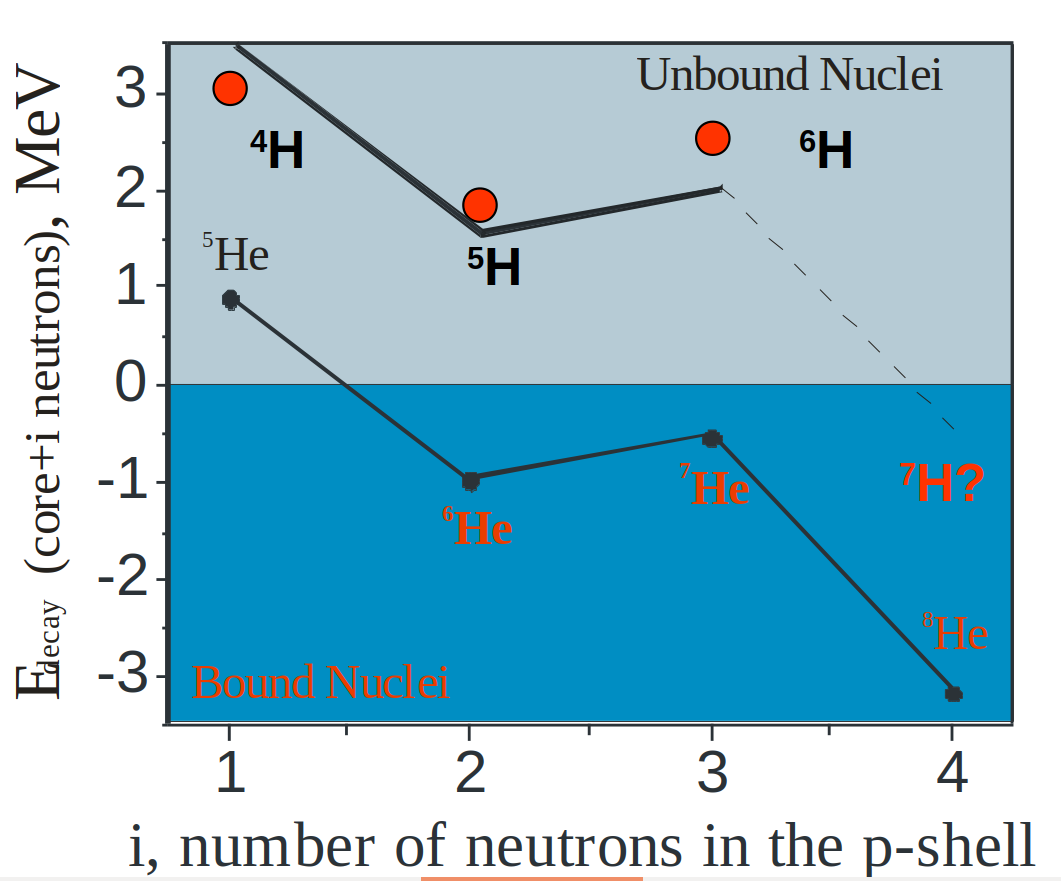
\includegraphics[width=0.49\textwidth]{figures/anomalie.png}
	\end{center}
	%
	\caption{Helium-hydrogen anomaly}
	%
	\label{fig:helium_anomaly}
\end{figure}
%-------------------------------------------------------------------------------

Calculations using the seven-body hyperspherical functions formalism \cite{Timofeyuk:2002} evaluated the $^{7}$H g.s.\ energy as $E_{T} \approx 0.84$\,MeV.
But at the same time, based on the assumption, that four valence neutrons of $^{7}$H occupy the same orbitals as in $^{8}$He, the simple estimations of the binding energy of the $^{7}$H ground state were performed in Ref.\ \cite{Korsheninnikov:2003}. 
The obtained value turned out to be $\approx 5.4$\,MeV, which means that this resonance state is expected at about 3\,MeV above the $^3$H+$4n$ decay threshold.
The authors also emphasized that the $^{7}$H ground state should undergo the unique five-body decay into $^3$H+$4n$ with very small width. 
Although, the experimental results of Ref.\ \cite{Korsheninnikov:2003} did not give a chance to identify any suggested states in a structure of $^{7}$H, the evidence of the $^{7}$H ground state resonance near the $^3$H+$4n$ decay threshold was obtained for the first time.
The MM spectrum of $^{7}$H obtained in that work showed a sharp increase starting from the $^3$H+$4n$ threshold.
This observation was important step towards solving the $^{7}$H problem, it did not allow the authors to give quantitative information about the resonance parameters because of low energy resolution (of $\approx 2$\,MeV) and complicated background conditions.

One should also mention the phenomenological estimates in Ref.\ \cite{Golovkov:2004} pointed to $E_{T} \approx 1.3-1.8$\,MeV.
The early pioneering theoretical works suffered from the low computation power and that is why mostly provided low quality estimations by kind of extrapolation methods.
This is clearly seen in works \cite{Aoyama:2004} and \cite{Aoyama:2009} where the same approach provided $E_{T} \approx 7$ and $E_{T} \approx 4$\,MeV respectively.
The authors used so-called antisymmetrized molecular dynamics (AMD) and gave analysis of the dineutron correlations in heavy helium and hydrogen isotopes.

The modern attempts of search for the superheavy hydrogen isotopes in the reaction of stopped pion absorbtion by light nuclei, are described in works Ref.\ \cite{Gurov:2007,Gurov:2009}.
In contrast to the early works \cite{Seth:1981,Evseev:1981}, the new approach was aimed to observe the short lived neutron rich resonances.
The missing mass method was used for reconstruction of the states of interest from the supposed reaction products.
The authors also conducted multiple correlation measurements of the same reaction mechanism, which allowed to ensure the applicability of this technique for neutron rich light isotopes and to determine the energy resolution of the obtained MM spectra, which turned out $\approx 3$\,MeV.
One searched $^7$H in the reactions $^{9}$B($\pi^-$,$p$$p$)$^7$H and $^{11}$B($\pi^-$,$p^3$He)$^7$H.
The count rate of the $p$+$^3$He products emitted in the $^{11}$B($\pi^-$,$p^3$He)$^7$H reaction was very low, which allowed only to observe the sharp rising of the MM spectrum near the $^3$H+$4n$ threshold.
Although such results indicated the existence of $^7$H as a resonance near the threshold of the supposed five-body breakup, the authors concluded that the $^{7}$H issue remains open.

The $^{7}$H existence was investigated by the authors of Refs.\ \cite{Caamano:2007,Caamano:2008} in the transfer reaction $^{12}$C($^{8}$He,$^{13}$N)$^{7}$H.
One considered the measurement of $^{13}$N in time-charge projection chamber (TPC) in coincidence with $^{3}$H detection by the segmented wall of cesium-iodide (CsI) scintillator detectors.
The obtained identification plots in works Refs.\ \cite{Caamano:2007,Caamano:2008} did not allow the authors to make the particle selections without risk of mixing up other elements.
Although in this work only seven events could be attributed to the desired reaction channel and despite to the declared poor $^{7}$H MM resolution of 2.5\,MeV for such low statistics, a very narrow $^7$H resonance was announced, with $E_T= 0.57^{+0.42}_{-0.21}$\,MeV.
It should be pointed out that, as far as nitrogen isotopes could not be identified inside the TPC, no actual reaction channel identification was possible in this experiment.
Moreover, the interpretation is essentially based on the assumption that only the $^{7}$H g.s.\ is populated in this reaction.
In reality, the population of the $^{7}$H excitation state is also possible in this experiment.
In addition, the reactions $^{12}$C($^{8}$He,$^{14}$N)$^{6}$H and $^{12}$C($^{8}$He,$^{15}$N)$^{5}$H may mock up the detection of $^{7}$H.

The authors of Ref.\ \cite{Fortier:2007} searched for the $^7$H in the $^2$H-$^3$He proton transfer reaction realized with $^8$He beam and CD$_{2}$ target. (Here and in the following, D$_2$ denotes
$^2$H$_2$.)
One should note, that due to relatively low beam energy of 15.3\,AMeV, the experimental acceptance covered only the energies up to 5\,MeV in the $^{7}$H excitation spectrum.
The plausibility of the obtained results were confirmed in conducted calibration runs, dedicated to production of the well known stable nuclei in reactions with the same mechanism.
Although, the detector system for the recoil $^3$He covered the large c.m. solid angle, the relatively poor MM energy resolution and low number of $^3$He-$^3$H coincidences did not allow to clearly observe any states in the obtained MM spectrum.
Although, in this work one concluded that there was an indication of a $^7$H resonance state in the measured MM spectrum at $E_T \approx 2$\,MeV, one should note, that within this narrow energy window, allowed for the $^{7}$H population, the obtained spectrum from the $^2$H($^8$He,$^3$He)$^7$H reaction looks very similar to the spectrum of the carbon-induced background from the CD$_2$ target, which made the authors cautious about their observations. 

The next attempt to discover $^{7}$H  using the already traditional reaction $^2$H($^8$He,$^3$He)$^7$H was made in Ref.\ \cite{Nikolskii:2010} at RIKEN.
As in the previous works, the reliability of the results, related to the system of interest, was tested by a reference experiment with $^2$H($^12$Be,$^3$He)$11$Li reaction.
The energy resolution of the MM spectrum, reconstructed from the low energy recoil $^3$He turned out to be $\approx 1.9$\,MeV.
The MM spectrum, reconstructed from $^3$He, demonstrated a rise at low energies, which cannot be reproduced with any continuum distribution concerning few-body phase space. 
However, no indication on the resonance peak was revealed in the measured $^7$H MM spectrum.
But it gave another evidence of the low energy resonance existence, close to the $^3$H+$4n$ decay threshold. 
Some peculiarity was found in the MM spectrum at $\approx 2$\,MeV, in addition, to another one at about 10.5\,MeV that could be a manifestation of a $^{7}$H continuum excitation.
The authors reported a value of about 30 $\mu$b/sr in c.m.\ for the cross-section of the reaction populating the low-energy part in the $^7$H spectrum, which, according to Distorted Wave Born Approximation (DWBA) calculations, turned out in contradiction with the announced in Ref.\ \cite{Caamano:2007} value.
The question of the reason of this discrepancy remained open, but in order to make the obtained results more plausible, the authors mentioned the work Ref.\ \cite{Aoyama:2009}, which showed, that due to the possible admixture of dineutron components in $^{7}$H.
Such effect doubts the assumption of the similarity of the valence nucleons in $^{7}$H and $^{8}$He due to a small overlap between their wave functions in the $^2$H($^8$He,$^3$He)$^7$H reaction, and that is why reduces its cross section.

Какие то слова что вопрос открыт
Но по крайней мере Для лёгких систем, прямые реакции - самые вероятные , и более того, чтобы достичь сильной ассиметрии массы и заряда, выбивание даже одного нуклона из RIB может быть достаточно получения системы за границей стабильности. Поэтому давайте использовать 8He. 

Можно заметить, что вопрос 7Н тесно связан с вопросом о существовании нейтронных кластеров. Были попытки описать .... и тд

\subsection{$^{6}$H studies}

Experimental information on the 6H resonant states is very limited.
The first significant experimental result on $^{6}$H was reported in Ref.\ \cite{Aleksandrov:1984}.
At that time, this system was supposed to be the heaviest possible hydrogen isotope and was searched in a complicated "bidirectional transfer" reaction $^7$Li($^7$Li,$^8$B)$^6$H.
Despite to the poor statistics and complicated background conditions, an evidence of $^{6}$H existence as a resonance at $E_T= 2.7\pm 0.4$\,MeV (above $^3$H+$3n$ decay threshold) was obtained for the first time.

Another pioneer experimental work Ref.\ \cite{Belozyorov:1986} described the attempt to produce the $^{6}$H resonance in the reaction $^9$Be($^{11}$B,$^{14}$O)$^6$H.
The authors declared the indication of the $^{6}$H existence as a low-lying resonance above the mentioned threshold population at $E_T= 2.6\pm 0.5$\,MeV, which turned out in good agreement with Ref.\ \cite{Aleksandrov:1984}.
However, one can note that in this experiment the energy range was strictly limited, which caused a kinematical cut-off of the provided spectrum.
That is why, the assigned controversial $^{6}$H state could be induced by this energy limitations.
Moreover, at the present moment, one can doubt these results, arguing that for some reason, already quite well known $^{5}$H was not observed in both pioneer experiments.

One should mention, that there have been attempts to search for $^{6}$H in a pion double exchange reaction Ref.\ \cite{PARKER:1990483}.
Such mechanism was realized in $^6$Li($\pi ^{-}$,$\pi ^{+}$)$^{6}$H reaction and allowed to explore the level
structure of $^{6}$H with high precision. 
But unfortunately, no data evidence for the $^{6}$H existence up to 30\,MeV above the decay threshold was found.
This observation brought serious doubts on the $^{6}$H existence, and as in the $^{7}$H case was a strong motivation to study $^{5}$H first.

The theoretical description of $^{6}$H is an extremely challenging task.
All the methods, which successfully worked out in the $^{5}$H case could not be applied for the $t+n+n+n$ system.
Even the seven-body hyperspherical functions formalism, realized in Ref.\ \cite{Timofeyuk:2002} did not allow to estimate the $^{6}$H energy, due to the computational obstacles.
The only one theoretical prediction, described in work Ref.\ \cite{Gorbatov:1989}, offered the energy of $6.3$\,MeV.
Also, similar results was obtained with the AMD approach applied in work Ref.\ \cite{Aoyama:2004}.
The authors evaluated the $^{6}$H g.s.\ energy as $E_{T} \approx 6$\,MeV, however, these both predictions did not satisfy any experimental results. 

The next conducted experiments were dedicated to the $^{6}$H search in the reaction of stopped pion absorbtion on $^{9}$Be and $^{11}$B targets and described in Ref.\ \cite{Gurov:2007}.
For the $^{6}$H structure reconstruction the MM method was used with determined resolution of 3\,MeV.
%The mass of triton plus three neutrons was used as a zero level.
The collected statistics was more than an order of magnitude higher, than in previous experiments, which allowed the authors reported the observation of few resonant states at $E_T = {6.6(7), 10.7(7), 15.3(7), 21.3(4)}$\,MeV for the first time.
However, in the first measurement with $^{9}$Be target, the lowest populated state at 6.6\,MeV was fitted to some distortion on the left slope of the 10.7\,MeV peak.
In the experimental run with $^{11}$B target the 10.7\,MeV state was not observed at all, while the 7.3\,MeV peak could be seen as consistent with the possible scale of statistical fluctuations.

The search for the $^{6}$H isotope, described in Ref.\ \cite{Caamano:2008}, was performed by impinging the $^{8}$He on the isobutane (C$_{4}$H$_{10}$) target.
The studied reaction channel was a "satellite" for the mentioned $^{7}$H experimental run.
As for the main $^{7}$H run, the was no reaction identification of the studied reaction channel, all the obtained events could belong to either $^{5}$H or $^{6}$H or $^{7}$H.
Therefore all three these MM spectra were reconstructed simultaneously.
The $^{6}$H g.s. energy was assigned in this work as 2.9(9)\,MeV with resonance width of 1.52\,MeV, which was consistent with the results of Ref.\ \cite{Aleksandrov:1984,Belozyorov:1986}. 


The search for the $^{6}$H resonant states is an exciting challenge in itself, however, here we face two important questions related also to our understanding of the neighboring systems.

\renewcommand{\labelenumi}{\roman{enumi}}
\begin{enumerate}
	\item 
	What are the decay mechanisms of $^{7}$H? 
	For example, it could be either the true $^{7}$H->$^{3}$H+4n decay, or sequential $^{7}$H->$^{5}$H\,g.s.+2n, or, else, the $^{7}$H->$^{6}$H\,g.s.+n decay, depending on the initial state of $^{7}$H and ground state energies of the $^{5,6}$H. 
	While for $^{4}$H and $^{5}$H there are some relatively modern data, the spectrum of $^{6}$H is too uncertain.
	\item 
	What is the decay mechanism of the $^{6}$H ground state?
	Intuitive vision of the situation, also confirmed by the theoretical estimates of this work, predict that the $^{6}$H\,g.s. decay is likely to have a sequential $^{6}$H->$^{5}$H\,g.s.+n -> $^{3}$H+3n character. 
	In such a situation, by studying the $^{6}$H decay, one also gains access to the decay properties of the $^{5}$H ground state.
\end{enumerate}
